\documentclass[border=5pt]{standalone}
\usepackage{tikz}
\usetikzlibrary{patterns}

\begin{document}
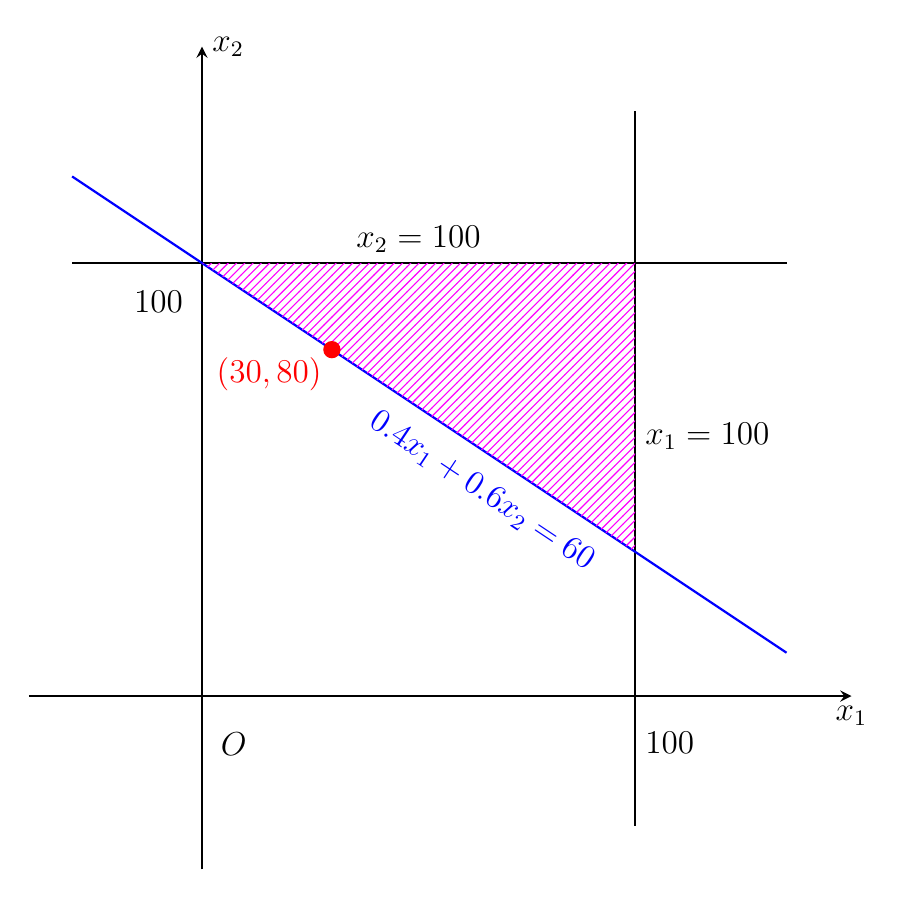
\begin{tikzpicture}[
    scale=0.055, 
    >=stealth, 
    line width=0.8pt,
    every node/.style={font=\large}
]
  
  % 1. 坐标轴与原点
  \draw[->] (-40,0) -- (150,0) node[below] {$x_1$};  % 横轴 x1
  \draw[->] (0,-40) -- (0,150) node[right] {$x_2$};  % 纵轴 x2
  \node[below right] at (2,-6) {$O$};                % 原点标注

  % 2. 约束边界线
  \draw (-30,100) -- (135,100);              % 水平约束线 x2 = 100
  \draw (100,-30) -- (100,135);              % 垂直约束线 x1 = 100
  % 倾斜约束线：0.4x1 + 0.6x2 = 60（标签沿直线倾斜并微调位置防重叠）
  \draw[blue] (-30,120) -- node[pos=0.6, below=4pt, sloped] {$0.4x_1+0.6x_2=60$} (135,10);

  % 3. 可行域（阴影网格区域）
  \fill[pattern=north east lines, pattern color=magenta] (0,100) -- (100,100) -- (100,33.3) -- cycle;

  % 4. 约束线与坐标轴刻度标注
  \node[above]       at (50,100)  {$x_2=100$};  % 顶部水平线标注
  \node[right]       at (100,60)  {$x_1=100$};  % 右侧垂直线标注
  \node[below right] at (100,-6)  {$100$};      % 横轴刻度 100
  \node[below left]  at (-2,96)   {$100$};      % 纵轴刻度 100

  % 5. 目标点 / 样本点标注
  \fill[red] (30,80) circle (2);
  \node[red, above left] at (30,68) {$(30,80)$}; % 点坐标文字
\end{tikzpicture}
\end{document}